 \documentclass{articleUL} 
 \usepackage[pdftex]{graphicx}
\usepackage{graphics}
\usepackage{amsmath}
\usepackage{color}
\usepackage{tikz}
\usepackage{titlesec}
\usepackage{hyperref}
\usepackage{pdfpages}
\usepackage{subfiles}
\titleclass{\subsubsubsection}{straight}[\subsection]

\newcounter{subsubsubsection}[subsubsection]
\renewcommand\thesubsubsubsection{\thesubsubsection.\arabic{subsubsubsection}}
\renewcommand\theparagraph{\thesubsubsubsection.\arabic{paragraph}} % optional; useful if paragraphs are to be numbered

\titleformat{\subsubsubsection}
  {\normalfont\normalsize\bfseries}{\thesubsubsubsection}{1em}{}
\titlespacing*{\subsubsubsection}
{0pt}{3.25ex plus 1ex minus .2ex}{1.5ex plus .2ex}

\makeatletter
\renewcommand\paragraph{\@startsection{paragraph}{5}{\z@}%
  {3.25ex \@plus1ex \@minus.2ex}%
  {-1em}%
  {\normalfont\normalsize\bfseries}}
\renewcommand\subparagraph{\@startsection{subparagraph}{6}{\parindent}%
  {3.25ex \@plus1ex \@minus .2ex}%
  {-1em}%
  {\normalfont\normalsize\bfseries}}
\def\toclevel@subsubsubsection{4}
\def\toclevel@paragraph{5}
\def\toclevel@paragraph{6}
\def\l@subsubsubsection{\@dottedtocline{4}{7em}{4em}}
\def\l@paragraph{\@dottedtocline{5}{10em}{5em}}
\def\l@subparagraph{\@dottedtocline{6}{14em}{6em}}
\makeatother

\setcounter{secnumdepth}{4}
\setcounter{tocdepth}{4}
\usetikzlibrary{positioning}
\usepackage{adjustbox}
\usepackage{float}
 \title{GMC-7004, Sujet Spécial (génie mécanique). Système d'exploitation de robot, ROS, environnement de simulation.} 
 %% You can add up to 7 differents authors
 \author{Philippe Lebel
 \affiliation{Université Laval, philippe.lebel.4@ulaval.ca}}
 \begin{document}
 \selectlanguage{french}	% Change to "francais" if needed
 \maketitle
 \subfile{abstract.tex}
 \newpage
 \subfile{intro.tex}
 \subfile{mise_contexte.tex}
 \subfile{Communication_ordinateur-robot.tex}
 \subfile{ur5_matlab.tex}
 \subfile{jaco_ros.tex}
 \begin{thebibliography}{}
 \bibitem{key1} First Reference...
 \bibitem{jaco_github} https://github.com/JenniferBuehler
 \end{thebibliography}
 \newpage
 \appendix
 \section{\\Exemple de code pour contrôle du bras Jaco sur Windows} \label{app:jaco_windows}

% the \\ insures the section title is centered below the phrase: Appendix A
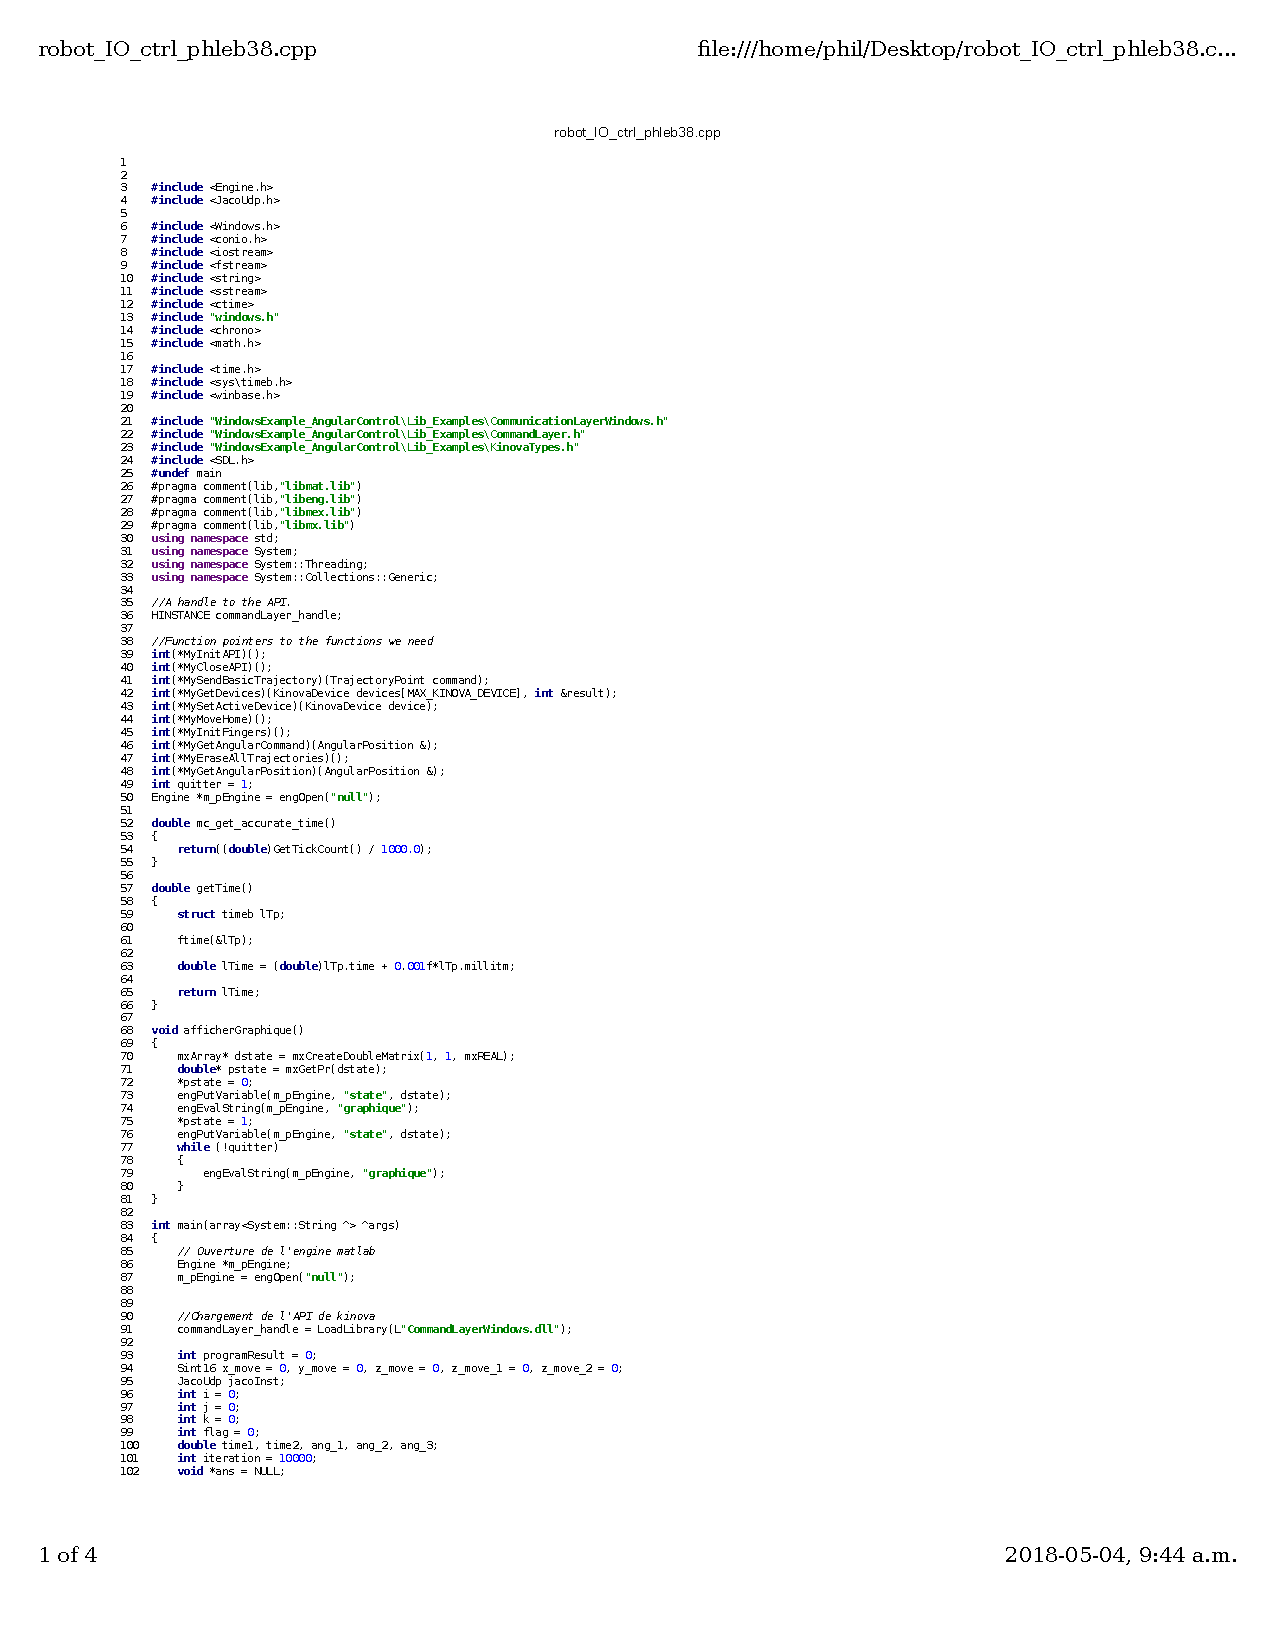
\includepdf[pages=-, offset=75 -75]{jaco_windows.pdf}
\section{\\Manuel de programmation URscript} \label{app:URscript_manual}

% the \\ insures the section title is centered below the phrase: Appendix A

\includepdf[pages=-, offset=75 -75]{scriptmanual_en_3_1.pdf}

\section{\\Fonctions de l'API VRep} \label{app:VRep_manual}

% the \\ insures the section title is centered below the phrase: Appendix A
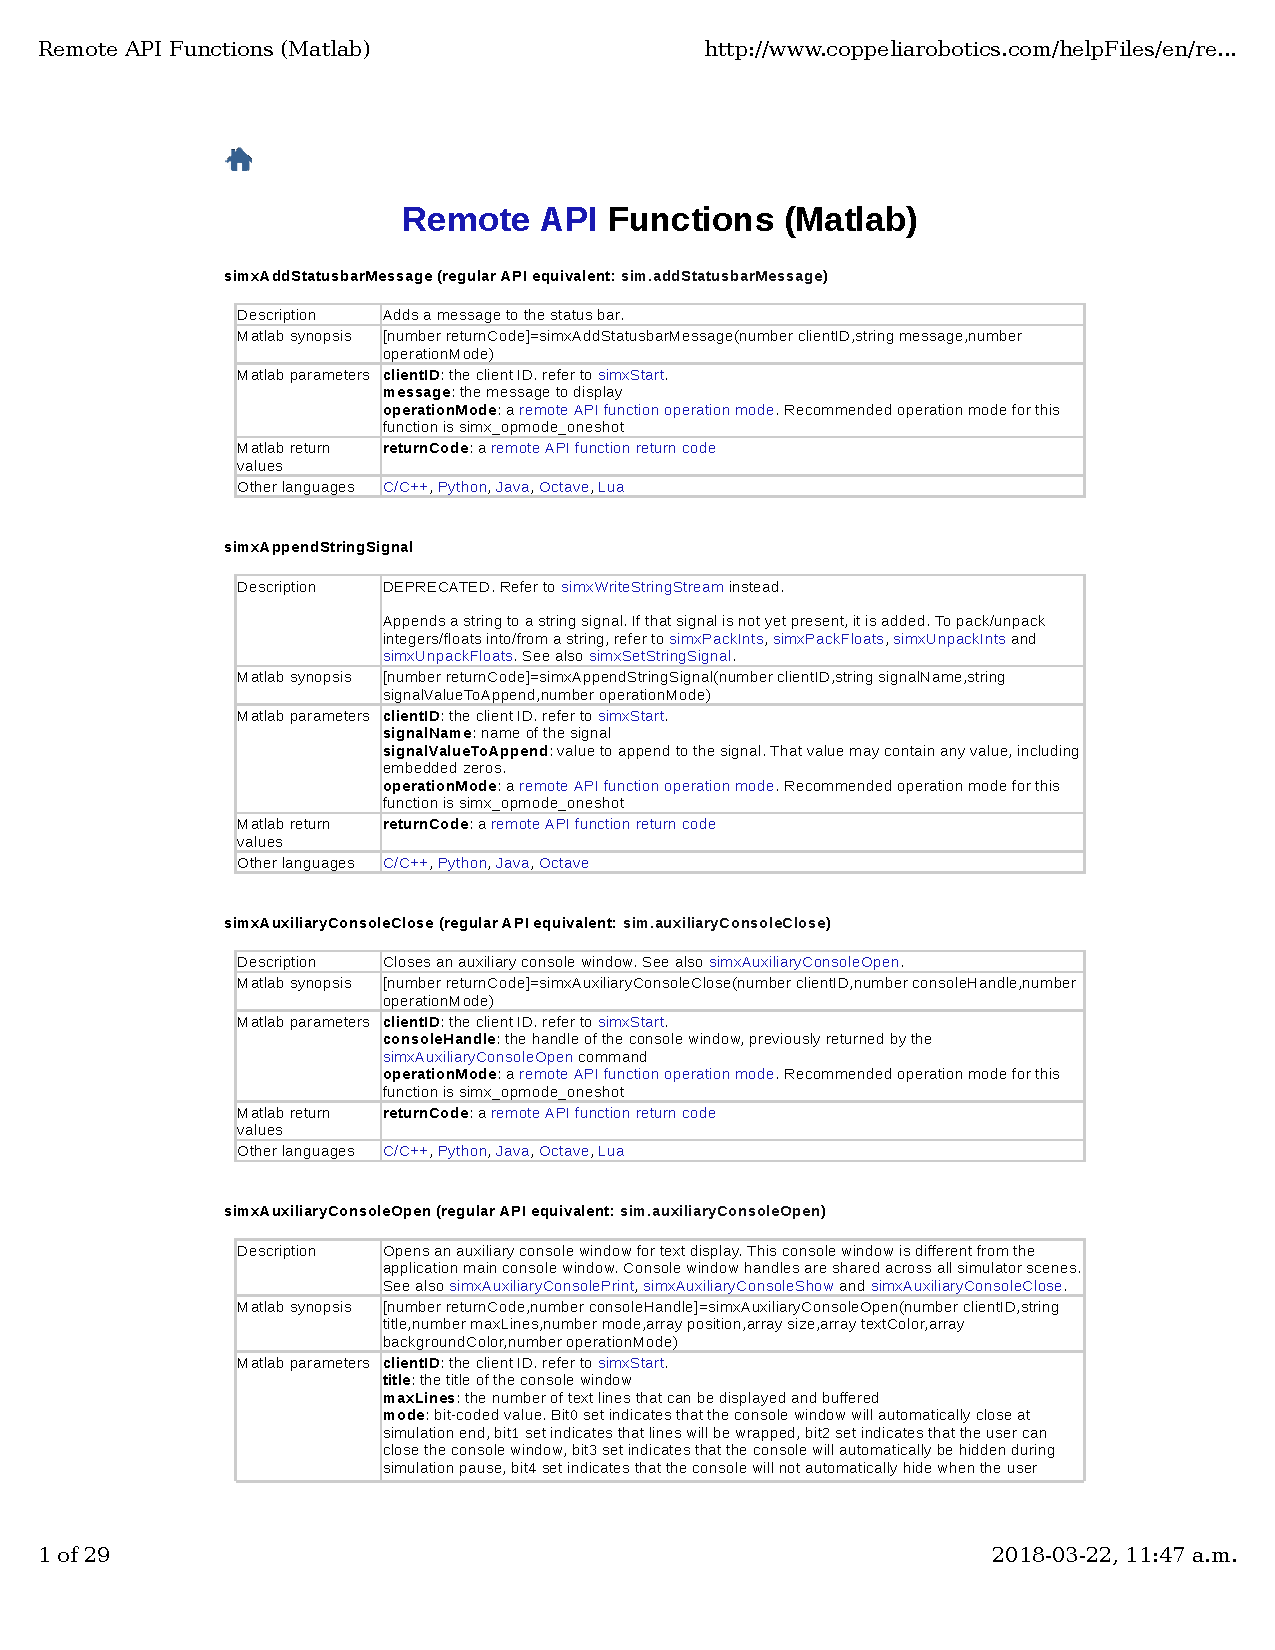
\includepdf[pages=-, offset=75 -75]{VRep_manual.pdf}
 \end{document} 